\chapter{Finite elements for transport problems}
\label{finitelements}

%%%%%%%%%%%%%%%%%%%%%%%%%%%%%%%%%%%%%%%%%%%%%%%%%%%%%%%%
%%%%%%%%%%%%%%%%%%%%%%%%%%%%%%%%%%%%%%%%%%%%%%%%%%%%%%%%
\section{General comments}
\label{sectgencom}

Consider transport of one medium. There is on quantity described by function $f$.
Flux of transported quantity depends on gradient of the function $f$. The function
$f$ is approximated in the form
\begin{equation}
f = \mbf{N} \mbf{d}
\end{equation}
where $\mbf{d}$ denotes nodal values of function $f$. Gradient of the function $f$ can be written as
\begin{equation}
\mbf{g} = {\rm grad}\ f = {\rm grad}\ \mbf{N} \mbf{d} = \mbf{B} \mbf{d}\ .
\end{equation}
From constitutive relation follows
\begin{equation}
\mbf{q} = \mbf{D} \mbf{g} = \mbf{D} \mbf{B} \mbf{d}
\end{equation}
where $\mbf{q}$ denotes flux. Finally, conservation law is used in form
\begin{equation}\label{eqconservlawelem}
{\rm div} \mbf{q} = {\rm div} \mbf{D} \mbf{B} \mbf{d} = 0\ .
\end{equation}
After application of Galerkin method which is based on premultiplication of (\ref{eqconservlawelem}) by test
function in form $\mbf{N}\mbf{d}$ and integration over solved domain, weak formulation is obtained in form
\begin{equation}
\int_{\Omega} \mbf{B}^T \mbf{D} \mbf{B} {\rm d}\Omega \mbf{d} = 0\ .
\end{equation}
Conductivity matrix of one finite element is defined as
\begin{equation}
\mbf{K} = \int_{\Omega} \mbf{B}^T \mbf{D} \mbf{B} {\rm d}\Omega
\end{equation}

More complicated situation is valid for several, say $n$, transported media. Fluxes of particular quantities
have form
\begin{equation}
\mbf{q}^i = \sum_{j=1}^n \mbf{D}_j^i \mbf{g}^j = \sum_{j=1}^n \mbf{D}_j^i \mbf{B}_j \mbf{d}_j\ .
\end{equation}
Each flux is used in conservation law
\begin{equation}
\forall i \in \{1,\ \ldots,\ n\}\ \ \ \ {\rm div} \mbf{q}^i = 0\ .
\end{equation}
New notation is defined for more simple handling with particular quantities. Matrices $\mbf{B}_j$
are located in one bigger matrix
\begin{equation}
\mbf{B} = \left(\begin{array}{cccc}
\mbf{B}_1 & \mbf{0}   & \ldots & \mbf{0}
\\
\mbf{0}   & \mbf{B}_2 &        & \vdots
\\
\vdots    &           & \ddots &
\\
\mbf{0}   & \ldots    &        & \mbf{B}_n
\end{array}\right)
\end{equation}
and vectors of nodal values are located in one vector
\begin{equation}
\mbf{d} = \left(\mbf{d}_1,\ \ldots,\ \mbf{d}_n\right)^T\ .
\end{equation}
Similar technique can be used for vectors of fluxes
\begin{equation}
\mbf{q} = \left(\mbf{q}_1,\ \ldots,\ \mbf{q}_n\right)^T\ .
\end{equation}
With this notation, constitutive relations can be expressed
\begin{equation}
\mbf{q} = \left(\begin{array}{c}
\mbf{q}_1
\\
\mbf{q}_2
\\
\vdots
\\
\mbf{q}_n
\end{array}\right) = \left(\begin{array}{cccc}
\mbf{D}_1^1 & \mbf{D}_2^1 & \ldots & \mbf{D}_n^1
\\
\mbf{D}_1^2 & \mbf{D}_2^2 &        & \mbf{D}_n^2
\\
\vdots      &             & \ddots & \vdots
\\
\mbf{D}_1^n & \mbf{D}_2^n & \ldots & \mbf{D}_n^n
\end{array}\right)
\left(\begin{array}{c}
\mbf{g}_1
\\
\mbf{g}_2
\\
\vdots
\\
\mbf{g}_n
\end{array}\right)
\end{equation}
Conservation laws require
\begin{equation}
\int_{\Omega} \mbf{B}^T \mbf{q} {\rm d}\Omega =
\int_{\Omega}
\left(\begin{array}{cccc}
\mbf{B}_1^T & \mbf{0}     & \ldots & \mbf{0}
\\
\mbf{0}     & \mbf{B}_2^T &        & \vdots
\\
\vdots      &             & \ddots &
\\
\mbf{0}     & \ldots      &        & \mbf{B}_n^T
\end{array}\right)
\left(\begin{array}{c}
\mbf{q}_1
\\
\mbf{q}_2
\\
\vdots
\\
\mbf{q}_n
\end{array}\right){\rm d}\Omega = \mbf{0}
\end{equation}
Conservation law can be rewritten
\begin{equation}
\int_{\Omega}
\left(\begin{array}{cccc}
\mbf{B}_1^T & \mbf{0}     & \ldots & \mbf{0}
\\
\mbf{0}     & \mbf{B}_2^T &        & \vdots
\\
\vdots      &             & \ddots &
\\
\mbf{0}     & \ldots      &        & \mbf{B}_n^T
\end{array}\right)
\left(\begin{array}{cccc}
\mbf{D}_1^1 & \mbf{D}_2^1 & \ldots & \mbf{D}_n^1
\\
\mbf{D}_1^2 & \mbf{D}_2^2 &        & \mbf{D}_n^2
\\
\vdots      &             & \ddots & \vdots
\\
\mbf{D}_1^n & \mbf{D}_2^n & \ldots & \mbf{D}_n^n
\end{array}\right)
\left(\begin{array}{c}
\mbf{B}_1\mbf{d}_1
\\
\mbf{B}_2\mbf{d}_2
\\
\vdots
\\
\mbf{B}_n\mbf{d}_n
\end{array}\right){\rm d}\Omega = \mbf{0}
\end{equation}
Conductivity matrix has form
\begin{equation}\label{condmatr}
\mbf{K} =
 \int_{\Omega}
\left(\begin{array}{cccc}
\mbf{B}_1^T \mbf{D}_1^1 \mbf{B}_1 & \mbf{B}_1^T \mbf{D}_2^1 \mbf{B}_2 & \ldots & \mbf{B}_1^T \mbf{D}_n^1 \mbf{B}_n
\\
\mbf{B}_2^T \mbf{D}_1^2 \mbf{B}_1 & \mbf{B}_2^T \mbf{D}_2^2 \mbf{B}_2 &        & \vdots
\\
\vdots                            &                                   & \ddots &
\\
\mbf{B}_n^T \mbf{D}_1^n \mbf{B}_1 & \mbf{B}_n^T \mbf{D}_2^n \mbf{B}_2 & \ldots & \mbf{B}_n^T \mbf{D}_n^n \mbf{B}_n
\end{array}\right)
{\rm d}\Omega
\end{equation}

%%%%%%%%%%%%%%%%%%%%%%%%%%%%%%%%%%%%%%%%%%%%%%%%%%%%%%%%
%%%%%%%%%%%%%%%%%%%%%%%%%%%%%%%%%%%%%%%%%%%%%%%%%%%%%%%%
\section{List of implemented finite elements}
\label{secfemlist}
\begin{itemize}
\item{2D bar element with linear approximation functions}
\item{2D bar element with quadratic approximation functions}
\item{triangular element with linear approximation functions}
\item{quadrilateral element with bi-linear approximation functions}
\item{plane quadrilateral element with bi-quadratic approximation functions}
\item{tetrahedral element with linear approximation functions}
\item{hexahedral element with tri-linear approximation functions}
\item{hexahedral element with tri-quadratic approximation functions}
\item{axisymmetric triangular element with linear approximation functions}
\item{axisymmetric quadrilateral element with bi-linear approximation functions}
\end{itemize}

%%%%%%%%%%%%%%%%%%%%%%%%%%%%%%%%%%%%%%%%%%%%%%%%%%%%%%%%
%%%%%%%%%%%%%%%%%%%%%%%%%%%%%%%%%%%%%%%%%%%%%%%%%%%%%%%%
\section{2D bar element with linear approximation functions}
\label{linbart}

\begin{center}
\begin{tabular}{|l|l|}
\hline
location & /TRFEL/SRC/linbart.cpp\\
         & /TRFEL/SRC/linbart.h
\\ \hline
number of blocks & 2
\\ \hline
block components & $(k), (c)$
\\ \hline
numer. integration & (2 int. points), (2 int. points)
\\ \hline
nodal DOF & number of transported media
\\ \hline
\end{tabular}
\end{center}

Approximation functions
\begin{eqnarray}
N_1^{(1)} &=& \del{1}{2}(1-\xi),\nonumber\\
N_2^{(1)} &=& \del{1}{2}(1+\xi),\nonumber\\
\ppd{N_1^{(1)}}{\xi} &=& -0.5,\\
\ppd{N_2^{(1)}}{\xi} &=& 0.5.\nonumber
\end{eqnarray}

%%%%%%%%%%%%%%%%%%%%%%%%%%%%%%%%%%%%%%%%%%%%%%%%%%%%%%%%
%%%%%%%%%%%%%%%%%%%%%%%%%%%%%%%%%%%%%%%%%%%%%%%%%%%%%%%%
\section{2D bar element with quadratic approximation functions}
\label{quadbart}

\begin{center}
\begin{tabular}{|l|l|}
\hline
location & /TRFEL/SRC/linbart.cpp\\
         & /TRFEL/SRC/linbart.h
\\ \hline
number of blocks & 2
\\ \hline
block components & $(k), (c)$
\\ \hline
numer. integration & (3 int. point), (3 int. points)
\\ \hline
nodal DOF & number of transported media
\\ \hline
\end{tabular}
\end{center}

Approximation functions
\begin{eqnarray}
N_1^{(1)} &=& \del{1}{2}\xi(\xi-1),\nonumber\\
N_2^{(1)} &=& \del{1}{2}\xi(1+\xi),\nonumber\\
N_3^{(1)} &=& 1-\xi^2,\\
\ppd{N_1^{(1)}}{\xi} &=& \xi-0.5,\nonumber\\
\ppd{N_2^{(1)}}{\xi} &=& \xi+0.5,\nonumber\\
\ppd{N_3^{(1)}}{\xi} &=& -2\xi.\nonumber
\end{eqnarray}

%%%%%%%%%%%%%%%%%%%%%%%%%%%%%%%%%%%%%%%%%%%%%%%%%%%%%%%%
%%%%%%%%%%%%%%%%%%%%%%%%%%%%%%%%%%%%%%%%%%%%%%%%%%%%%%%%
\section{Triangular element with linear approximation functions}
\label{trlint}

\begin{center}
\begin{tabular}{|l|l|}
\hline
location & /TRFEL/SRC/linbart.cpp\\
         & /TRFEL/SRC/linbart.h
\\ \hline
number of blocks & 2
\\ \hline
block components & $(k), (c)$
\\ \hline
numer. integration & (1 int. point), (3 int. points)
\\ \hline
nodal DOF & number of transported media
\\ \hline
\end{tabular}
\end{center}

Approximation functions
\begin{eqnarray}
N_1^{(1)} &=& L_1,\nonumber\\
N_2^{(1)} &=& L_2,\nonumber\\
N_3^{(1)} &=& 1-L_1-L_2,
\end{eqnarray}

For more details about approximation functions see GEFEL~\ref{}.

%%%%%%%%%%%%%%%%%%%%%%%%%%%%%%%%%%%%%%%%%%%%%%%%%%%%%%%%
%%%%%%%%%%%%%%%%%%%%%%%%%%%%%%%%%%%%%%%%%%%%%%%%%%%%%%%%
\section{Quadrilateral element with bi-linear approximation functions}
\label{quadlint}

\begin{center}
\begin{tabular}{|l|l|}
\hline
location & /TRFEL/SRC/linbart.cpp\\
         & /TRFEL/SRC/linbart.h
\\ \hline
number of blocks & 2
\\ \hline
block components & $(k), (c)$
\\ \hline
numer. integration & ($2 \times 2$ points), ($2 \times 2$ points)
\\ \hline
nodal DOF & number of transported media
\\ \hline
\end{tabular}
\end{center}

For details about approximation functions see GEFEL~\ref{}.

%%%%%%%%%%%%%%%%%%%%%%%%%%%%%%%%%%%%%%%%%%%%%%%%%%%%%%%%
%%%%%%%%%%%%%%%%%%%%%%%%%%%%%%%%%%%%%%%%%%%%%%%%%%%%%%%%
\section{Quadrilateral element with bi-quadratic approximation functions}
\label{quadquadt}

\begin{center}
\begin{tabular}{|l|l|}
\hline
location & /TRFEL/SRC/linbart.cpp\\
         & /TRFEL/SRC/linbart.h
\\ \hline
number of blocks & 2
\\ \hline
block components & $(k), (c)$
\\ \hline
numer. integration & ($3 \times 3$ points), ($3 \times 3$ points)
\\ \hline
nodal DOF & number of transported media
\\ \hline
\end{tabular}
\end{center}

For details about approximation functions see GEFEL~\ref{}.

%%%%%%%%%%%%%%%%%%%%%%%%%%%%%%%%%%%%%%%%%%%%%%%%%%%%%%%%
%%%%%%%%%%%%%%%%%%%%%%%%%%%%%%%%%%%%%%%%%%%%%%%%%%%%%%%%
\section{Tetrahedral element with linear approximation functions}
\label{lintett}

\begin{center}
\begin{tabular}{|l|l|}
\hline
location & /TRFEL/SRC/linbart.cpp\\
         & /TRFEL/SRC/linbart.h
\\ \hline
number of blocks & 2
\\ \hline
block components & $(k), (c)$
\\ \hline
numer. integration & (1 int. point), (4 int. points)
\\ \hline
nodal DOF & number of transported media
\\ \hline
\end{tabular}
\end{center}

Approximation functions
\begin{eqnarray}
N_1^{(1)} &=& L_1,\nonumber\\
N_2^{(1)} &=& L_2,\nonumber\\
N_3^{(1)} &=& L_3,\\
N_4^{(1)} &=& 1-L_1-L_2-L_3,\nonumber
\end{eqnarray}

For more details about approximation functions see GEFEL~\ref{}.

%%%%%%%%%%%%%%%%%%%%%%%%%%%%%%%%%%%%%%%%%%%%%%%%%%%%%%%%
%%%%%%%%%%%%%%%%%%%%%%%%%%%%%%%%%%%%%%%%%%%%%%%%%%%%%%%%
\section{Hexahedral element with tri-linear approximation functions}
\label{linhext}

\begin{center}
\begin{tabular}{|l|l|}
\hline
location & /TRFEL/SRC/linbart.cpp\\
         & /TRFEL/SRC/linbart.h
\\ \hline
number of blocks & 2
\\ \hline
block components & $(k), (c)$
\\ \hline
numer. integration & ($2 \times 2 \times 2$ points), ($2 \times 2 \times 2$ points)
\\ \hline
nodal DOF & number of transported media
\\ \hline
\end{tabular}
\end{center}

For details about approximation functions see GEFEL~\ref{}.

%%%%%%%%%%%%%%%%%%%%%%%%%%%%%%%%%%%%%%%%%%%%%%%%%%%%%%%%
%%%%%%%%%%%%%%%%%%%%%%%%%%%%%%%%%%%%%%%%%%%%%%%%%%%%%%%%
\section{Hexahedral element with tri-quadratic approximation functions}
\label{hexquadt}

\begin{center}
\begin{tabular}{|l|l|}
\hline
location & /TRFEL/SRC/linbart.cpp\\
         & /TRFEL/SRC/linbart.h
\\ \hline
number of blocks & 2
\\ \hline
block components & $(k), (c)$
\\ \hline
numer. integration & ($3 \times 3 \times 3$ points), ($3 \times 3 \times 3$ points)
\\ \hline
nodal DOF & number of transported media
\\ \hline
\end{tabular}
\end{center}

For details about approximation functions see GEFEL~\ref{}.

%%%%%%%%%%%%%%%%%%%%%%%%%%%%%%%%%%%%%%%%%%%%%%%%%%%%%%%%
%%%%%%%%%%%%%%%%%%%%%%%%%%%%%%%%%%%%%%%%%%%%%%%%%%%%%%%%
\section{Axisymmetric domain}

We can simplify the 3D formulation into the axisymmetric one under the assumption that the axisymmetric body 
is subject to axisymmetric boundary conditions.

\begin{figure}[h!]
\begin{center}
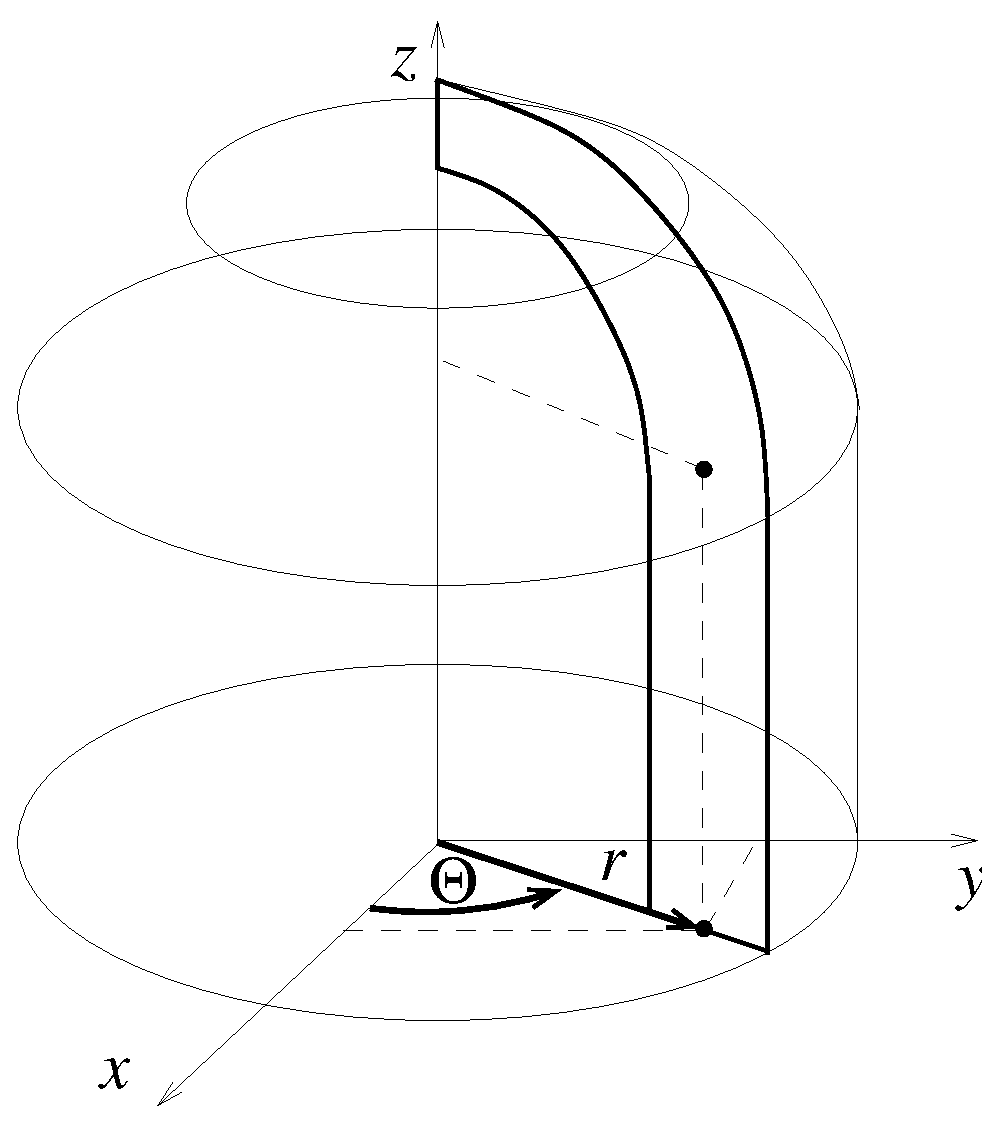
\includegraphics[angle=0, width=6.5cm]{PS/note_axisym.eps}
\caption{Notation for axisymmetric domain}
\label{axisym}
\end{center}
\end{figure}

We start by modifying integral \eqref{nkint}, in which partial derivatives of general shape functions 
$\tenss{N}$ expressed in axisymmetric coordinates (Fig. \ref{axisym}) take this form
\begin{eqnarray}\label{der_ax}
\frac{\partial \tenss{N}}{\partial x} &=&  \frac{\partial \tenss{N}}{\partial r} \frac{\partial r}{\partial x} 
+ \frac{\partial \tenss{N}}{\partial \Theta} \frac{\partial \Theta}{\partial x},\nonumber\\
\frac{\partial\tenss{N} }{\partial y} &=&  \frac{\partial\tenss{N} }{\partial r} \frac{\partial r}{\partial y} 
+ \frac{\partial \tenss{N}}{\partial \Theta} \frac{\partial \Theta}{\partial y},\\
\frac{\partial \tenss{N}}{\partial z} &=&  \frac{\partial \tenss{N}}{\partial z}\nonumber,\\
{\rm d} \Omega &=& {\rm d}x \;{\rm d}y \;{\rm d}z = r \;{\rm d}\Theta \;{\rm d}r \;{\rm d}z,\nonumber
\end{eqnarray}
where
\begin{eqnarray}\label{der_gon}
\frac{\partial r}{\partial x} = \cos \Theta,\quad
\frac{\partial r}{\partial y} = \sin \Theta,\quad
\frac{\partial \Theta}{\partial x} = -\frac{\sin \Theta}{r},\quad
\frac{\partial r}{\partial y} = \frac{\cos \Theta}{r}.
\end{eqnarray}
The first two Eqs.~\eqref{der_ax} can be rewritten as:
\begin{eqnarray}\label{der_n}
\frac{\partial \tenss{N}}{\partial x} =  \frac{\partial \tenss{N}}{\partial r} \cos \Theta 
- \frac{\partial \tenss{N}}{\partial \Theta} \frac{\sin \Theta}{r},\nonumber\\
\frac{\partial \tenss{N}}{\partial y} =  \frac{\partial \tenss{N}}{\partial r} \sin \Theta 
+ \frac{\partial \tenss{N}}{\partial \Theta} \frac{\cos \Theta}{r}.
\end{eqnarray}
Application of Eqs.~\eqref{der_ax} and \eqref{der_n} and subsequent mathematical operations,
lead to integrals expressing the conductivity matrix
\begin{eqnarray}\label{n_int}
\tenss{K} &=& \int_{\Omega} \Big(\frac{\partial \tenss{N}^T}{\partial r} k
\frac{\partial \tenss{N}}{\partial r} \cos^2 \Theta
+ \frac{\partial \tenss{N}^T}{\partial r}k\frac{\partial \tenss{N}}{\partial r} \sin^2 \Theta + 
\frac{\partial \tenss{N}^T}{\partial z}k\frac{\partial \tenss{N}}{\partial z}\Big)
r \;{\rm d}\Theta \;{\rm d}r \;{\rm d}z = \nonumber\\
&=&\int_{\Omega} \Big(\frac{\partial \tenss{N}^T}{\partial r}k\frac{\partial \tenss{N}}{\partial r} + 
\frac{\partial \tenss{N}^T}{\partial z}k\frac{\partial \tenss{N}}{\partial z}\Big)
r \;{\rm d}\Theta \;{\rm d}r \;{\rm d}z,
\end{eqnarray}
where $\tenss{N}$ represents the shape functions of variables $u$ and $k$ stands for the 
material variable. 
The resulting integral formula for the conductivity matrix is obtained after integration 
of \eqref{n_int} with respect to $\Theta$ from 0 to 2$\pi$.
\begin{eqnarray}\label{int_k}
\tenss{K} &=& 2\pi \int_{\Omega} \Big(\frac{\partial \tenss{N}^T}{\partial r}k\frac{\partial \tenss{N}}{\partial r} + 
\frac{\partial \tenss{N}^T}{\partial z}k\frac{\partial \tenss{N}}{\partial z}\Big)
r \;{\rm d}r \;{\rm d}z.
\end{eqnarray}
The capacity matrix and vectors of prescribed fluxes can be treated in a similar manner.
\begin{eqnarray}
\tenss{C} = 2\pi \int_{\Omega} \Big( \tenss{N}^T c\ \tenss{N}\Big) r \;{\rm d}r \;{\rm d}z ,
\end{eqnarray}
\begin{eqnarray}
\overline{\tenss{q}} = 2\pi \int_{\Gamma} \Big(\tenss{N}_q^T  \overline{q}\Big) r \;{\rm d}r \;{\rm d}z,
\end{eqnarray}
where $\overline{q}$ corresponds to the prescribed fluxes.

%%%%%%%%%%%%%%%%%%%%%%%%%%%%%%%%%%%%%%%%%%%%%%%%%%%%%%%%
\subsection{Axisymmetric triangular element with linear approximation functions}
\label{trlaxt}

\begin{center}
\begin{tabular}{|l|l|}
\hline
location & /TRFEL/SRC/linbart.cpp\\
         & /TRFEL/SRC/linbart.h
\\ \hline
number of blocks & 2
\\ \hline
block components & $(k), (c)$
\\ \hline
numer. integration & (1 int. point), (3 int. points)
\\ \hline
nodal DOF & number of transported media
\\ \hline
\end{tabular}
\end{center}

Approximation functions
\begin{eqnarray}
N_1^{(1)} &=& L_1,\nonumber\\
N_2^{(1)} &=& L_2,\nonumber\\
N_3^{(1)} &=& 1-L_1-L_2,
\end{eqnarray}

For more details about approximation functions see GEFEL~\ref{}.

%%%%%%%%%%%%%%%%%%%%%%%%%%%%%%%%%%%%%%%%%%%%%%%%%%%%%%%%
\subsection{Axisymmetric quadrilateral element with bi-linear approximation functions}
\label{qualaxt}


\begin{center}
\begin{tabular}{|l|l|}
\hline
location & /TRFEL/SRC/linbart.cpp\\
         & /TRFEL/SRC/linbart.h
\\ \hline
number of blocks & 2
\\ \hline
block components & $(k), (c)$
\\ \hline
numer. integration & ($2 \times 2$ points), ($2 \times 2$ points)
\\ \hline
nodal DOF & number of transported media
\\ \hline
\end{tabular}
\end{center}

Approximation functions

\begin{eqnarray}
N_1^{(1)} &=& \del{1}{4} (1 + \xi) (1 + \eta),\nonumber\\
N_2^{(1)} &=& \del{1}{4} (1 - \xi) (1 + \eta),\nonumber\\
N_3^{(1)} &=& \del{1}{4} (1 - \xi) (1 - \eta),\nonumber\\
N_4^{(1)} &=& \del{1}{4} (1 + \xi) (1 - \eta),\\
\ppd{N_1^{(1)}}{\xi} &=& \del{1}{4} (1 + \eta),\nonumber\\
\ppd{N_2^{(1)}}{\xi} &=& - \del{1}{4} (1 + \eta),\nonumber\\
\ppd{N_3^{(1)}}{\xi} &=& - \del{1}{4} (1 - \eta),\nonumber\\
\ppd{N_4^{(1)}}{\xi} &=& \del{1}{4} (1 - \eta),\nonumber\\
\ppd{N_1^{(1)}}{\eta} &=& \del{1}{4} (1 + \xi),\nonumber\\
\ppd{N_2^{(1)}}{\eta} &=& \del{1}{4} (1 - \xi),\nonumber\\
\ppd{N_3^{(1)}}{\eta} &=& - \del{1}{4} (1 - \xi),\nonumber\\
\ppd{N_4^{(1)}}{\eta} &=& - \del{1}{4} (1 + \xi).\nonumber
\end{eqnarray}
